%%__________________________________________________________________||
\section{Introduction}
\label{sec:introduction}


Astronomical observations have determined that 27\% of our Universe’s energy content is composed of an unknown form of matter - dark matter (DM) - that is entirely different from normal matter that contributes just 5\%. DM has yet been only observed in gravitationally and its precise nature remains one of the most important discoveries in fundamental physics. Astrophysical measurements indicate that DM consists of very weakly interacting particles at a scale potentially accessible at the Large Hadron Collider (LHC). Of several complementary detection approaches potential collider production offers particularly good sensitivity at low DM masses and offer complementary sensitivity at larger masses while not being  subject to astrophysical uncertainties. Collider searches are also largely independent to the spin-structure of the interaction and can potentially access particle like heavy quarks that might be suppressed in direct or indirect DM searches.



This document presents an inclusive search for the pair production of WIMPs in hadronic final states with two or more
energetic jets and \met, performed in pp collisions at a centre-of-mass energy $\sqrt{s} = 13\TeV$. The analysed data sample
corresponds to an integrated luminosity of $2.1 \pm 0.15 \fbinv$~\cite{lumi} collected by the Compact Muon Solenoid (CMS)
experiment. Previous iterations of this search have been performed in
pp collisions at both $\sqrt{s} = 7$~\cite{RA1Paper, RA1Paper2011, RA1Paper2011FULL} and $8\TeV$~\cite{RA1Paper2012}.

Interpretations of the analysis are provided in the parameter space of simplified models~\cite{Alwall:2008ag, Alwall:2008va, sms}. Limits are derived in the mass parameter space of simplified models of pair-produced gluinos, decaying inclusively to four quarks and addtionally decaying to four top and bottom quarks. Figure~\ref{fig:feyn} illustrates the simplified models considered.

\begin{figure*}[thb]
\centering
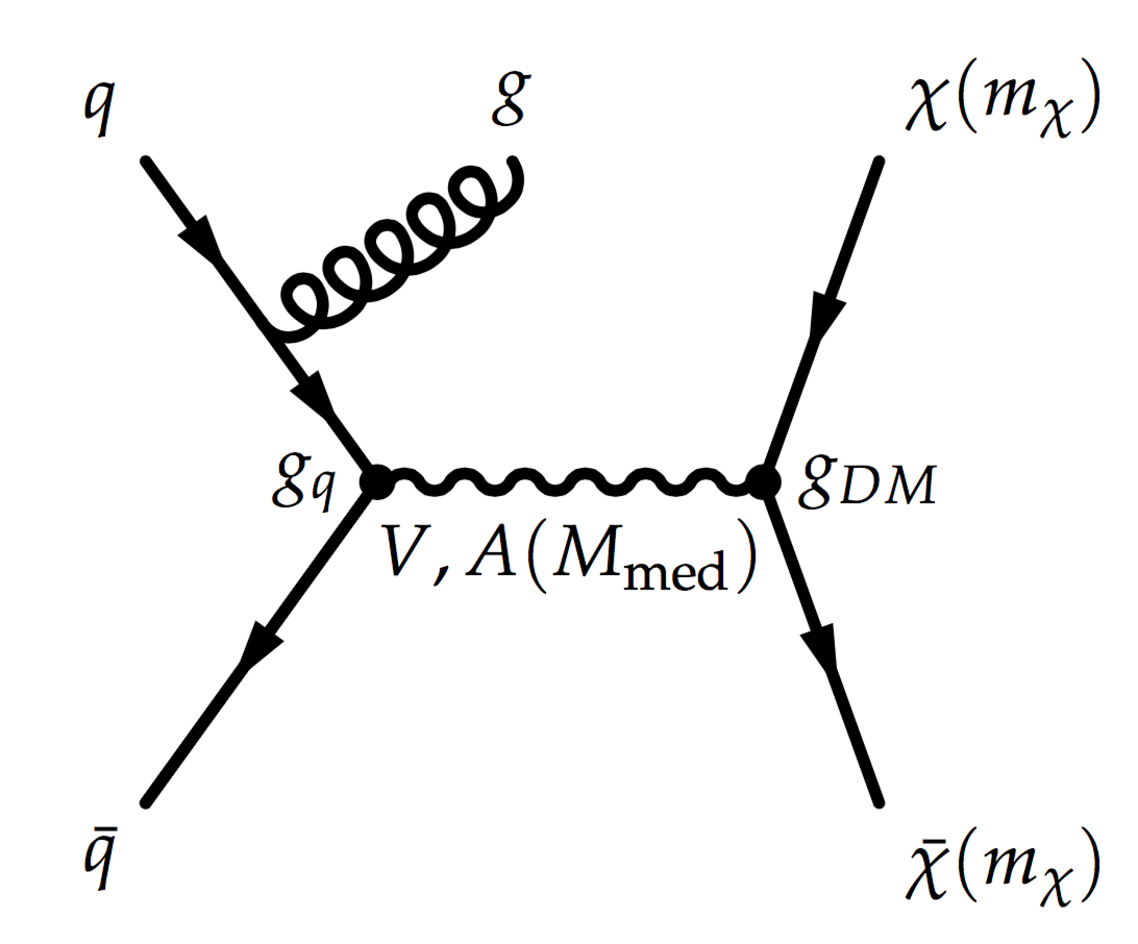
\includegraphics[width=0.4\linewidth]{feynman_light_jet.pdf}
\hfill
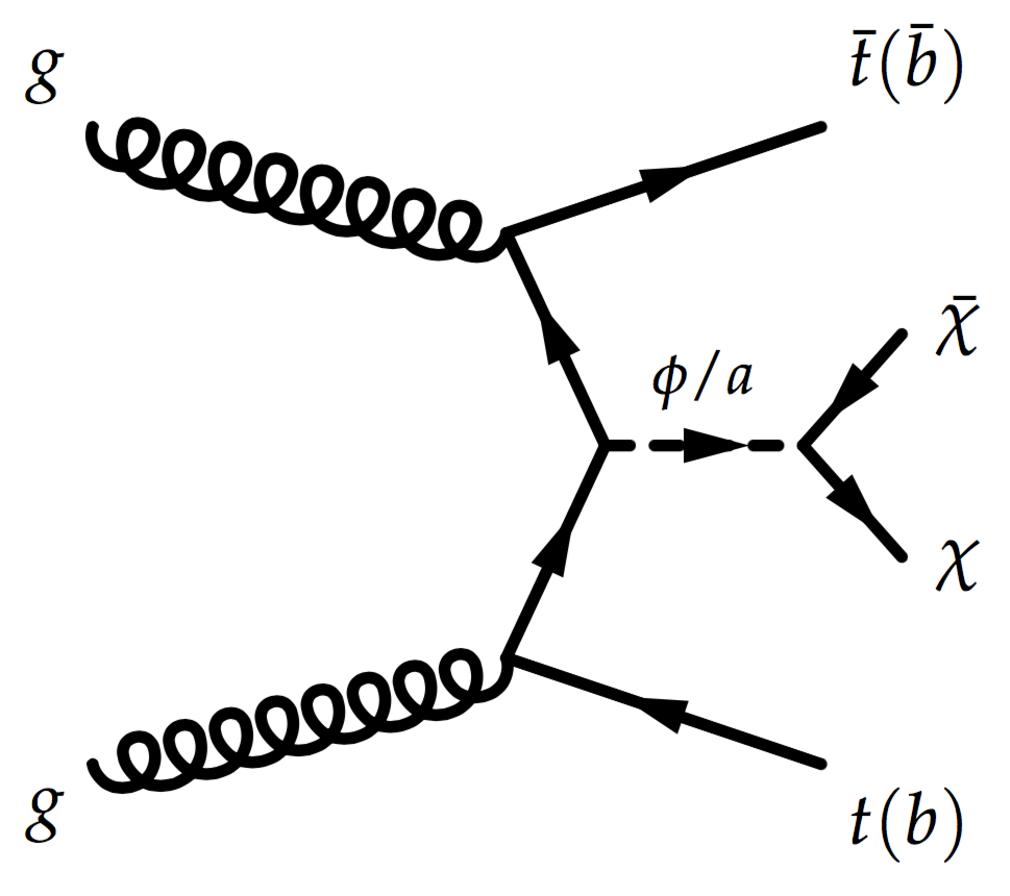
\includegraphics[width=0.35\linewidth]{feynman_hf.pdf}
\caption{Feynman diagrams for the minimal simplified DM models for light quarks (left) and heavy quarks}
\label{fig:feyn}
\end{figure*}

The search is devised around the kinematic variable \alphat that provides powerful discrimination against multijet production, a
manifestation of quantum chromodynamics (QCD), and adheres to an inclusive strategy with the aim of providing sensitivity to the widest possible range of DM models. The \alphat variable is constructed from jet-based quantities to provide robust discriminating power between sources of genuine and misreconstructed missing energy, making it suitable for early searches.

The search is based on an examination of the number of reconstructed jets per event, the scalar and vector sums of
transverse energies of these jets, and the number of these jets identified as originating from bottom quarks. 

%%__________________________________________________________________||
